% Created by tikzDevice version 0.12.6 on 2024-02-26 22:02:24
% !TEX encoding = UTF-8 Unicode
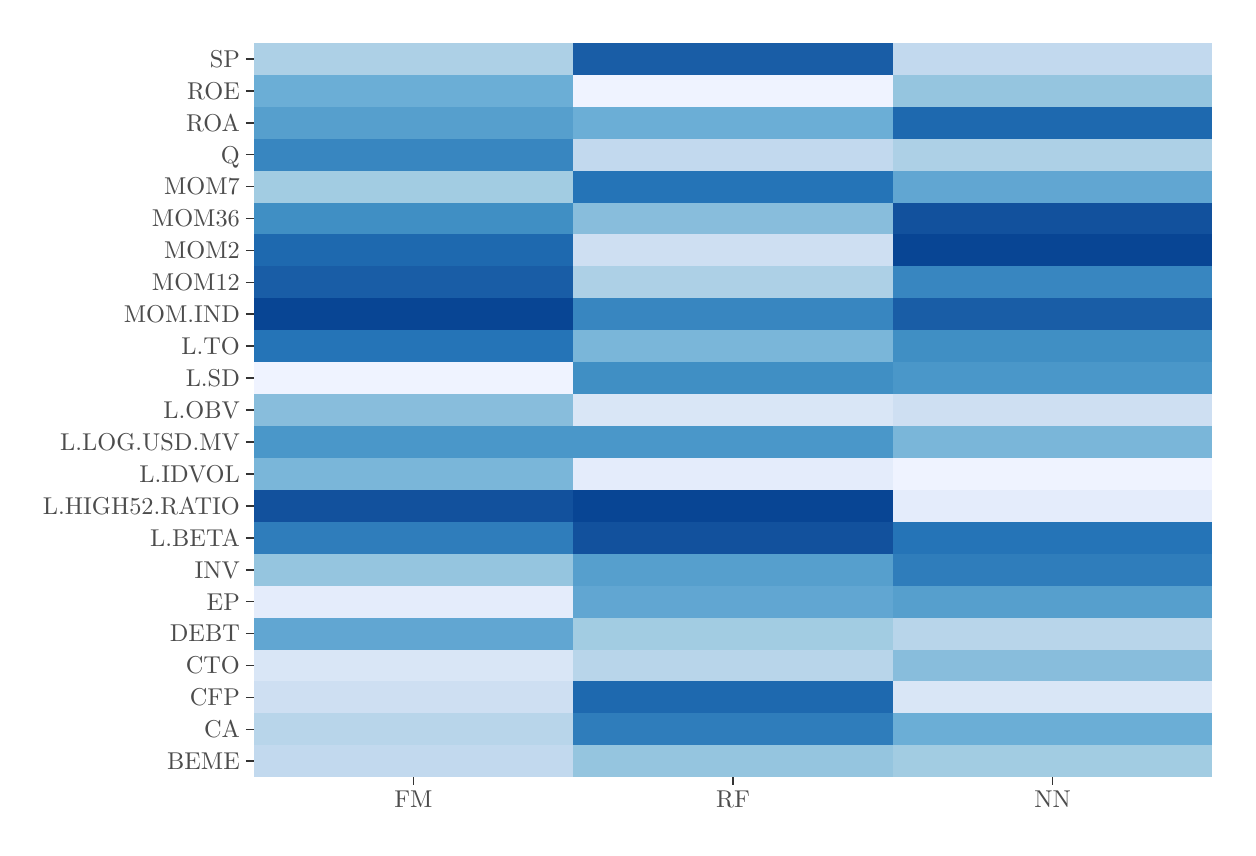
\begin{tikzpicture}[x=1pt,y=1pt]
\definecolor{fillColor}{RGB}{255,255,255}
\path[use as bounding box,fill=fillColor,fill opacity=0.00] (0,0) rectangle (433.62,289.08);
\begin{scope}
\path[clip] (  0.00,  0.00) rectangle (433.62,289.08);
\definecolor{drawColor}{RGB}{255,255,255}
\definecolor{fillColor}{RGB}{255,255,255}

\path[draw=drawColor,line width= 0.6pt,line join=round,line cap=round,fill=fillColor] (  0.00,  0.00) rectangle (433.62,289.08);
\end{scope}
\begin{scope}
\path[clip] ( 81.63, 18.22) rectangle (428.12,283.58);
\definecolor{fillColor}{gray}{0.92}

\path[fill=fillColor] ( 81.63, 18.22) rectangle (428.12,283.58);
\definecolor{drawColor}{RGB}{255,255,255}

\path[draw=drawColor,line width= 0.6pt,line join=round] ( 81.63, 23.99) --
	(428.12, 23.99);

\path[draw=drawColor,line width= 0.6pt,line join=round] ( 81.63, 35.53) --
	(428.12, 35.53);

\path[draw=drawColor,line width= 0.6pt,line join=round] ( 81.63, 47.06) --
	(428.12, 47.06);

\path[draw=drawColor,line width= 0.6pt,line join=round] ( 81.63, 58.60) --
	(428.12, 58.60);

\path[draw=drawColor,line width= 0.6pt,line join=round] ( 81.63, 70.14) --
	(428.12, 70.14);

\path[draw=drawColor,line width= 0.6pt,line join=round] ( 81.63, 81.68) --
	(428.12, 81.68);

\path[draw=drawColor,line width= 0.6pt,line join=round] ( 81.63, 93.21) --
	(428.12, 93.21);

\path[draw=drawColor,line width= 0.6pt,line join=round] ( 81.63,104.75) --
	(428.12,104.75);

\path[draw=drawColor,line width= 0.6pt,line join=round] ( 81.63,116.29) --
	(428.12,116.29);

\path[draw=drawColor,line width= 0.6pt,line join=round] ( 81.63,127.83) --
	(428.12,127.83);

\path[draw=drawColor,line width= 0.6pt,line join=round] ( 81.63,139.36) --
	(428.12,139.36);

\path[draw=drawColor,line width= 0.6pt,line join=round] ( 81.63,150.90) --
	(428.12,150.90);

\path[draw=drawColor,line width= 0.6pt,line join=round] ( 81.63,162.44) --
	(428.12,162.44);

\path[draw=drawColor,line width= 0.6pt,line join=round] ( 81.63,173.98) --
	(428.12,173.98);

\path[draw=drawColor,line width= 0.6pt,line join=round] ( 81.63,185.51) --
	(428.12,185.51);

\path[draw=drawColor,line width= 0.6pt,line join=round] ( 81.63,197.05) --
	(428.12,197.05);

\path[draw=drawColor,line width= 0.6pt,line join=round] ( 81.63,208.59) --
	(428.12,208.59);

\path[draw=drawColor,line width= 0.6pt,line join=round] ( 81.63,220.12) --
	(428.12,220.12);

\path[draw=drawColor,line width= 0.6pt,line join=round] ( 81.63,231.66) --
	(428.12,231.66);

\path[draw=drawColor,line width= 0.6pt,line join=round] ( 81.63,243.20) --
	(428.12,243.20);

\path[draw=drawColor,line width= 0.6pt,line join=round] ( 81.63,254.74) --
	(428.12,254.74);

\path[draw=drawColor,line width= 0.6pt,line join=round] ( 81.63,266.27) --
	(428.12,266.27);

\path[draw=drawColor,line width= 0.6pt,line join=round] ( 81.63,277.81) --
	(428.12,277.81);

\path[draw=drawColor,line width= 0.6pt,line join=round] (139.38, 18.22) --
	(139.38,283.58);

\path[draw=drawColor,line width= 0.6pt,line join=round] (254.87, 18.22) --
	(254.87,283.58);

\path[draw=drawColor,line width= 0.6pt,line join=round] (370.37, 18.22) --
	(370.37,283.58);
\definecolor{fillColor}{RGB}{149,197,223}

\path[fill=fillColor] (197.12, 18.22) rectangle (312.62, 29.76);
\definecolor{fillColor}{RGB}{47,125,187}

\path[fill=fillColor] (197.12, 29.76) rectangle (312.62, 41.30);
\definecolor{fillColor}{RGB}{30,105,175}

\path[fill=fillColor] (197.12, 41.30) rectangle (312.62, 52.83);
\definecolor{fillColor}{RGB}{184,213,234}

\path[fill=fillColor] (197.12, 52.83) rectangle (312.62, 64.37);
\definecolor{fillColor}{RGB}{162,204,226}

\path[fill=fillColor] (197.12, 64.37) rectangle (312.62, 75.91);
\definecolor{fillColor}{RGB}{97,166,210}

\path[fill=fillColor] (197.12, 75.91) rectangle (312.62, 87.45);
\definecolor{fillColor}{RGB}{86,159,205}

\path[fill=fillColor] (197.12, 87.45) rectangle (312.62, 98.98);
\definecolor{fillColor}{RGB}{18,81,157}

\path[fill=fillColor] (197.12, 98.98) rectangle (312.62,110.52);
\definecolor{fillColor}{RGB}{8,69,148}

\path[fill=fillColor] (197.12,110.52) rectangle (312.62,122.06);
\definecolor{fillColor}{RGB}{228,236,251}

\path[fill=fillColor] (197.12,122.06) rectangle (312.62,133.59);
\definecolor{fillColor}{RGB}{74,151,201}

\path[fill=fillColor] (197.12,133.59) rectangle (312.62,145.13);
\definecolor{fillColor}{RGB}{217,230,246}

\path[fill=fillColor] (197.12,145.13) rectangle (312.62,156.67);
\definecolor{fillColor}{RGB}{64,143,196}

\path[fill=fillColor] (197.12,156.67) rectangle (312.62,168.21);
\definecolor{fillColor}{RGB}{122,182,217}

\path[fill=fillColor] (197.12,168.21) rectangle (312.62,179.74);
\definecolor{fillColor}{RGB}{56,134,192}

\path[fill=fillColor] (197.12,179.74) rectangle (312.62,191.28);
\definecolor{fillColor}{RGB}{173,208,230}

\path[fill=fillColor] (197.12,191.28) rectangle (312.62,202.82);
\definecolor{fillColor}{RGB}{206,223,242}

\path[fill=fillColor] (197.12,202.82) rectangle (312.62,214.36);
\definecolor{fillColor}{RGB}{136,189,220}

\path[fill=fillColor] (197.12,214.36) rectangle (312.62,225.89);
\definecolor{fillColor}{RGB}{37,116,183}

\path[fill=fillColor] (197.12,225.89) rectangle (312.62,237.43);
\definecolor{fillColor}{RGB}{194,217,238}

\path[fill=fillColor] (197.12,237.43) rectangle (312.62,248.97);
\definecolor{fillColor}{RGB}{107,174,214}

\path[fill=fillColor] (197.12,248.97) rectangle (312.62,260.51);
\definecolor{fillColor}{RGB}{239,243,255}

\path[fill=fillColor] (197.12,260.51) rectangle (312.62,272.04);
\definecolor{fillColor}{RGB}{25,93,166}

\path[fill=fillColor] (197.12,272.04) rectangle (312.62,283.58);
\definecolor{fillColor}{RGB}{194,217,238}

\path[fill=fillColor] ( 81.63, 18.22) rectangle (197.12, 29.76);
\definecolor{fillColor}{RGB}{184,213,234}

\path[fill=fillColor] ( 81.63, 29.76) rectangle (197.12, 41.30);
\definecolor{fillColor}{RGB}{206,223,242}

\path[fill=fillColor] ( 81.63, 41.30) rectangle (197.12, 52.83);
\definecolor{fillColor}{RGB}{217,230,246}

\path[fill=fillColor] ( 81.63, 52.83) rectangle (197.12, 64.37);
\definecolor{fillColor}{RGB}{97,166,210}

\path[fill=fillColor] ( 81.63, 64.37) rectangle (197.12, 75.91);
\definecolor{fillColor}{RGB}{228,236,251}

\path[fill=fillColor] ( 81.63, 75.91) rectangle (197.12, 87.45);
\definecolor{fillColor}{RGB}{149,197,223}

\path[fill=fillColor] ( 81.63, 87.45) rectangle (197.12, 98.98);
\definecolor{fillColor}{RGB}{47,125,187}

\path[fill=fillColor] ( 81.63, 98.98) rectangle (197.12,110.52);
\definecolor{fillColor}{RGB}{18,81,157}

\path[fill=fillColor] ( 81.63,110.52) rectangle (197.12,122.06);
\definecolor{fillColor}{RGB}{122,182,217}

\path[fill=fillColor] ( 81.63,122.06) rectangle (197.12,133.59);
\definecolor{fillColor}{RGB}{74,151,201}

\path[fill=fillColor] ( 81.63,133.59) rectangle (197.12,145.13);
\definecolor{fillColor}{RGB}{136,189,220}

\path[fill=fillColor] ( 81.63,145.13) rectangle (197.12,156.67);
\definecolor{fillColor}{RGB}{239,243,255}

\path[fill=fillColor] ( 81.63,156.67) rectangle (197.12,168.21);
\definecolor{fillColor}{RGB}{37,116,183}

\path[fill=fillColor] ( 81.63,168.21) rectangle (197.12,179.74);
\definecolor{fillColor}{RGB}{8,69,148}

\path[fill=fillColor] ( 81.63,179.74) rectangle (197.12,191.28);
\definecolor{fillColor}{RGB}{25,93,166}

\path[fill=fillColor] ( 81.63,191.28) rectangle (197.12,202.82);
\definecolor{fillColor}{RGB}{30,105,175}

\path[fill=fillColor] ( 81.63,202.82) rectangle (197.12,214.36);
\definecolor{fillColor}{RGB}{64,143,196}

\path[fill=fillColor] ( 81.63,214.36) rectangle (197.12,225.89);
\definecolor{fillColor}{RGB}{162,204,226}

\path[fill=fillColor] ( 81.63,225.89) rectangle (197.12,237.43);
\definecolor{fillColor}{RGB}{56,134,192}

\path[fill=fillColor] ( 81.63,237.43) rectangle (197.12,248.97);
\definecolor{fillColor}{RGB}{86,159,205}

\path[fill=fillColor] ( 81.63,248.97) rectangle (197.12,260.51);
\definecolor{fillColor}{RGB}{107,174,214}

\path[fill=fillColor] ( 81.63,260.51) rectangle (197.12,272.04);
\definecolor{fillColor}{RGB}{173,208,230}

\path[fill=fillColor] ( 81.63,272.04) rectangle (197.12,283.58);
\definecolor{fillColor}{RGB}{162,204,226}

\path[fill=fillColor] (312.62, 18.22) rectangle (428.12, 29.76);
\definecolor{fillColor}{RGB}{107,174,214}

\path[fill=fillColor] (312.62, 29.76) rectangle (428.12, 41.30);
\definecolor{fillColor}{RGB}{217,230,246}

\path[fill=fillColor] (312.62, 41.30) rectangle (428.12, 52.83);
\definecolor{fillColor}{RGB}{136,189,220}

\path[fill=fillColor] (312.62, 52.83) rectangle (428.12, 64.37);
\definecolor{fillColor}{RGB}{184,213,234}

\path[fill=fillColor] (312.62, 64.37) rectangle (428.12, 75.91);
\definecolor{fillColor}{RGB}{86,159,205}

\path[fill=fillColor] (312.62, 75.91) rectangle (428.12, 87.45);
\definecolor{fillColor}{RGB}{47,125,187}

\path[fill=fillColor] (312.62, 87.45) rectangle (428.12, 98.98);
\definecolor{fillColor}{RGB}{37,116,183}

\path[fill=fillColor] (312.62, 98.98) rectangle (428.12,110.52);
\definecolor{fillColor}{RGB}{228,236,251}

\path[fill=fillColor] (312.62,110.52) rectangle (428.12,122.06);
\definecolor{fillColor}{RGB}{239,243,255}

\path[fill=fillColor] (312.62,122.06) rectangle (428.12,133.59);
\definecolor{fillColor}{RGB}{122,182,217}

\path[fill=fillColor] (312.62,133.59) rectangle (428.12,145.13);
\definecolor{fillColor}{RGB}{206,223,242}

\path[fill=fillColor] (312.62,145.13) rectangle (428.12,156.67);
\definecolor{fillColor}{RGB}{74,151,201}

\path[fill=fillColor] (312.62,156.67) rectangle (428.12,168.21);
\definecolor{fillColor}{RGB}{64,143,196}

\path[fill=fillColor] (312.62,168.21) rectangle (428.12,179.74);
\definecolor{fillColor}{RGB}{25,93,166}

\path[fill=fillColor] (312.62,179.74) rectangle (428.12,191.28);
\definecolor{fillColor}{RGB}{56,134,192}

\path[fill=fillColor] (312.62,191.28) rectangle (428.12,202.82);
\definecolor{fillColor}{RGB}{8,69,148}

\path[fill=fillColor] (312.62,202.82) rectangle (428.12,214.36);
\definecolor{fillColor}{RGB}{18,81,157}

\path[fill=fillColor] (312.62,214.36) rectangle (428.12,225.89);
\definecolor{fillColor}{RGB}{97,166,210}

\path[fill=fillColor] (312.62,225.89) rectangle (428.12,237.43);
\definecolor{fillColor}{RGB}{173,208,230}

\path[fill=fillColor] (312.62,237.43) rectangle (428.12,248.97);
\definecolor{fillColor}{RGB}{30,105,175}

\path[fill=fillColor] (312.62,248.97) rectangle (428.12,260.51);
\definecolor{fillColor}{RGB}{149,197,223}

\path[fill=fillColor] (312.62,260.51) rectangle (428.12,272.04);
\definecolor{fillColor}{RGB}{194,217,238}

\path[fill=fillColor] (312.62,272.04) rectangle (428.12,283.58);
\end{scope}
\begin{scope}
\path[clip] (  0.00,  0.00) rectangle (433.62,289.08);
\definecolor{drawColor}{gray}{0.30}

\node[text=drawColor,anchor=base east,inner sep=0pt, outer sep=0pt, scale=  0.88] at ( 76.68, 20.96) {BEME};

\node[text=drawColor,anchor=base east,inner sep=0pt, outer sep=0pt, scale=  0.88] at ( 76.68, 32.50) {CA};

\node[text=drawColor,anchor=base east,inner sep=0pt, outer sep=0pt, scale=  0.88] at ( 76.68, 44.03) {CFP};

\node[text=drawColor,anchor=base east,inner sep=0pt, outer sep=0pt, scale=  0.88] at ( 76.68, 55.57) {CTO};

\node[text=drawColor,anchor=base east,inner sep=0pt, outer sep=0pt, scale=  0.88] at ( 76.68, 67.11) {DEBT};

\node[text=drawColor,anchor=base east,inner sep=0pt, outer sep=0pt, scale=  0.88] at ( 76.68, 78.65) {EP};

\node[text=drawColor,anchor=base east,inner sep=0pt, outer sep=0pt, scale=  0.88] at ( 76.68, 90.18) {INV};

\node[text=drawColor,anchor=base east,inner sep=0pt, outer sep=0pt, scale=  0.88] at ( 76.68,101.72) {L.BETA};

\node[text=drawColor,anchor=base east,inner sep=0pt, outer sep=0pt, scale=  0.88] at ( 76.68,113.26) {L.HIGH52.RATIO};

\node[text=drawColor,anchor=base east,inner sep=0pt, outer sep=0pt, scale=  0.88] at ( 76.68,124.80) {L.IDVOL};

\node[text=drawColor,anchor=base east,inner sep=0pt, outer sep=0pt, scale=  0.88] at ( 76.68,136.33) {L.LOG.USD.MV};

\node[text=drawColor,anchor=base east,inner sep=0pt, outer sep=0pt, scale=  0.88] at ( 76.68,147.87) {L.OBV};

\node[text=drawColor,anchor=base east,inner sep=0pt, outer sep=0pt, scale=  0.88] at ( 76.68,159.41) {L.SD};

\node[text=drawColor,anchor=base east,inner sep=0pt, outer sep=0pt, scale=  0.88] at ( 76.68,170.95) {L.TO};

\node[text=drawColor,anchor=base east,inner sep=0pt, outer sep=0pt, scale=  0.88] at ( 76.68,182.48) {MOM.IND};

\node[text=drawColor,anchor=base east,inner sep=0pt, outer sep=0pt, scale=  0.88] at ( 76.68,194.02) {MOM12};

\node[text=drawColor,anchor=base east,inner sep=0pt, outer sep=0pt, scale=  0.88] at ( 76.68,205.56) {MOM2};

\node[text=drawColor,anchor=base east,inner sep=0pt, outer sep=0pt, scale=  0.88] at ( 76.68,217.09) {MOM36};

\node[text=drawColor,anchor=base east,inner sep=0pt, outer sep=0pt, scale=  0.88] at ( 76.68,228.63) {MOM7};

\node[text=drawColor,anchor=base east,inner sep=0pt, outer sep=0pt, scale=  0.88] at ( 76.68,240.17) {Q};

\node[text=drawColor,anchor=base east,inner sep=0pt, outer sep=0pt, scale=  0.88] at ( 76.68,251.71) {ROA};

\node[text=drawColor,anchor=base east,inner sep=0pt, outer sep=0pt, scale=  0.88] at ( 76.68,263.24) {ROE};

\node[text=drawColor,anchor=base east,inner sep=0pt, outer sep=0pt, scale=  0.88] at ( 76.68,274.78) {SP};
\end{scope}
\begin{scope}
\path[clip] (  0.00,  0.00) rectangle (433.62,289.08);
\definecolor{drawColor}{gray}{0.20}

\path[draw=drawColor,line width= 0.6pt,line join=round] ( 78.88, 23.99) --
	( 81.63, 23.99);

\path[draw=drawColor,line width= 0.6pt,line join=round] ( 78.88, 35.53) --
	( 81.63, 35.53);

\path[draw=drawColor,line width= 0.6pt,line join=round] ( 78.88, 47.06) --
	( 81.63, 47.06);

\path[draw=drawColor,line width= 0.6pt,line join=round] ( 78.88, 58.60) --
	( 81.63, 58.60);

\path[draw=drawColor,line width= 0.6pt,line join=round] ( 78.88, 70.14) --
	( 81.63, 70.14);

\path[draw=drawColor,line width= 0.6pt,line join=round] ( 78.88, 81.68) --
	( 81.63, 81.68);

\path[draw=drawColor,line width= 0.6pt,line join=round] ( 78.88, 93.21) --
	( 81.63, 93.21);

\path[draw=drawColor,line width= 0.6pt,line join=round] ( 78.88,104.75) --
	( 81.63,104.75);

\path[draw=drawColor,line width= 0.6pt,line join=round] ( 78.88,116.29) --
	( 81.63,116.29);

\path[draw=drawColor,line width= 0.6pt,line join=round] ( 78.88,127.83) --
	( 81.63,127.83);

\path[draw=drawColor,line width= 0.6pt,line join=round] ( 78.88,139.36) --
	( 81.63,139.36);

\path[draw=drawColor,line width= 0.6pt,line join=round] ( 78.88,150.90) --
	( 81.63,150.90);

\path[draw=drawColor,line width= 0.6pt,line join=round] ( 78.88,162.44) --
	( 81.63,162.44);

\path[draw=drawColor,line width= 0.6pt,line join=round] ( 78.88,173.98) --
	( 81.63,173.98);

\path[draw=drawColor,line width= 0.6pt,line join=round] ( 78.88,185.51) --
	( 81.63,185.51);

\path[draw=drawColor,line width= 0.6pt,line join=round] ( 78.88,197.05) --
	( 81.63,197.05);

\path[draw=drawColor,line width= 0.6pt,line join=round] ( 78.88,208.59) --
	( 81.63,208.59);

\path[draw=drawColor,line width= 0.6pt,line join=round] ( 78.88,220.12) --
	( 81.63,220.12);

\path[draw=drawColor,line width= 0.6pt,line join=round] ( 78.88,231.66) --
	( 81.63,231.66);

\path[draw=drawColor,line width= 0.6pt,line join=round] ( 78.88,243.20) --
	( 81.63,243.20);

\path[draw=drawColor,line width= 0.6pt,line join=round] ( 78.88,254.74) --
	( 81.63,254.74);

\path[draw=drawColor,line width= 0.6pt,line join=round] ( 78.88,266.27) --
	( 81.63,266.27);

\path[draw=drawColor,line width= 0.6pt,line join=round] ( 78.88,277.81) --
	( 81.63,277.81);
\end{scope}
\begin{scope}
\path[clip] (  0.00,  0.00) rectangle (433.62,289.08);
\definecolor{drawColor}{gray}{0.20}

\path[draw=drawColor,line width= 0.6pt,line join=round] (139.38, 15.47) --
	(139.38, 18.22);

\path[draw=drawColor,line width= 0.6pt,line join=round] (254.87, 15.47) --
	(254.87, 18.22);

\path[draw=drawColor,line width= 0.6pt,line join=round] (370.37, 15.47) --
	(370.37, 18.22);
\end{scope}
\begin{scope}
\path[clip] (  0.00,  0.00) rectangle (433.62,289.08);
\definecolor{drawColor}{gray}{0.30}

\node[text=drawColor,anchor=base,inner sep=0pt, outer sep=0pt, scale=  0.88] at (139.38,  7.21) {FM};

\node[text=drawColor,anchor=base,inner sep=0pt, outer sep=0pt, scale=  0.88] at (254.87,  7.21) {RF};

\node[text=drawColor,anchor=base,inner sep=0pt, outer sep=0pt, scale=  0.88] at (370.37,  7.21) {NN};
\end{scope}
\end{tikzpicture}
